%% Template for Master thesis
%% ===========================
%%
%% You need at least KomaScript v3.0.0,
%% e.g. available in Texlive 2009
\documentclass  [
  paper    = a4,
  BCOR     = 10mm,
  twoside,
  fontsize = 12pt,
  fleqn,
  toc      = bibnumbered,
  toc      = listofnumbered,
  numbers  = noendperiod,
  headings = normal,
  listof   = leveldown,
  version  = 3.03
]                                       {scrreprt}

% used pagages
\usepackage     [utf8]                  {inputenc}
\usepackage     [T1]                    {fontenc}
\usepackage                             {color}
\usepackage                             {amsmath}
\usepackage                             {graphicx}
\usepackage     [english]               {babel}
\usepackage                             {natbib}
\usepackage                             {hyperref}

% links
\definecolor{darkblue}{rgb}{0.0,0.0,0.4}
\definecolor{darkgreen}{rgb}{0.0,0.4,0.0}
\hypersetup{
    colorlinks,
    linkcolor=black,
    citecolor=darkgreen,
    urlcolor=darkblue
}

\begin{document}
  %% title pages similar to providet template instead of maketitle
  %% Titelseiten ähnlich zum Layout des Formulars von der
%% Fakultät für Physik und Astronomie
%%
%% Weitere Infos:
%% http://www.physik.uni-heidelberg.de/aktuelles/studium/
%% (PDF link: ...studium/download/145/Vorlage_Diplomarbeit_Formular.pdf)

%% Titelintro
\thispagestyle{empty}
\begin{center}
  \renewcommand{\baselinestretch}{2.00}
  \Large\sffamily
  Fakult\"{a}t f\"{u}r Physik und Astronomie\\
  \large
  Ruprecht-Karls-Universit\"{a}t Heidelberg
  \par\vfill\normalfont
  Masterarbeit\\
  Im Studiengang Physik\\
  vorgelegt von\\
  (Vor- und Zuname)\\
  geboren in (Geburtsort)\\
  (Jahr der Abgabe)\\
\end{center}
\newpage

%% Titelseite
\thispagestyle{empty}
\begin{center}
  \renewcommand{\baselinestretch}{2.00}
  \Large\bfseries\sffamily
    (Titel)\\
    (der)\\
    (Masterarbeit)
  \par
  \vfill
  \large\normalfont
  Die Masterarbeit wurde von (Vorname Name)\\
  ausgef\"{u}hrt am\\
  (Institut)\\
  unter der Betreuung von\\
  (Frau/Herrn Prof./Priv.-Doz. Vorname Name)
  %% Bei externen Masterarbeiten hier noch den zweiten Betreuer einfügen
  %% und den vspace in Z. 45 entsprechend reduzieren
\end{center}\par
\vspace{5\baselineskip}

% Zeilenabstand zurücksetzen
\renewcommand{\baselinestretch}{1.00}\normalsize % select either german
  %% this will generate title pages similar to the template provided
%% by the Department of Physics and Astronomy Heidelberg
%%
%% More information:
%% http://www.physik.uni-heidelberg.de/aktuelles/studium/
%% (PDF link: ...studium/download/145/Vorlage_Diplomarbeit_Formular.pdf)

%% Titleintro
\thispagestyle{empty}
\begin{center}
  \renewcommand{\baselinestretch}{2.00}
  \Large\sffamily
  Department of Physics and Astronomy\\
  \large University of Heidelberg
  \par\vfill\normalfont
  Master thesis\\
  in Physics\\
  submitted by\\
  Jacob Nieswand\\
  born in Konstanz\\
  2018
\end{center}
\newpage

%% Titlepage
\thispagestyle{empty}
\begin{center}
  \renewcommand{\baselinestretch}{2.00}
  \Large\bfseries\sffamily
    Optimizations of Light Field measurements\\
    using the structure tensor
  \par
  \vfill
  \large\normalfont
  This Master thesis has been carried out by Jacob Nieswand\\
  at the\\
  Institut für wissenschaftliches Rechnen (IWR)\\
  under the supervision of\\
  Herrn Priv.-Doz. Christoph Garbe
  %% additionally insert second supervisor here if carrying out an
  %% external diploma thesis. Reduce vspace in L. 44 accordingly.
\end{center}\par
\vspace{5\baselineskip}

% reset baselinestretch
\renewcommand{\baselinestretch}{1.00}\normalsize % or english title page
  %% Abstract page
%% =============
%%
%% Content of abstract pages has been put into seperate pages to simplify
%% word counting. Use e.g. the unix command
%%   wc abstract-ger.tex
%% or
%%   wc abstract-eng.tex
%% to get the number of words contained in these files.
\thispagestyle{empty}
\begin{center}
  \begin{minipage}[c][0.48\textheight][b]{0.9\textwidth}
    \small
    \textbf{
      Optimierung von EPI-basierten Lichtfeldmessungen:
    }\par
    \vspace{\baselineskip}
    
Diese Arbeit befasst sich mit der Tiefenrekonstruktion einer Szene mittels 2D-Aufnahmen aus verschiedenen Blickwinkeln (Lichtfeld). Aus der Struktur der epipolaren Schnitte durch das Lichtfeld (EPIs) wird mithilfe des Strukturtensors die Tiefe errechnet. In dieser Arbeit werden verschiedene Modifikationen bestehender entwickelter Algorithmen getestet, weiterhin werden Depth-of-defocus- Techniken getestet und verglichen. Zusätzlich wird ein Algorithmus basierend auf dem in der Stereo-Vision verbreiteten Semi-global Matching Algorithmus (SGM) als Nachbearbeitungsschritt implementiert.
  \end{minipage}\par
  \vfill
  \begin{minipage}[c][0.48\textheight][b]{0.9\textwidth}
    \small
    \textbf{
      (Title of Master thesis - english):
    }\par
    \vspace{\baselineskip}
    This work deas with 3D depth reconstruction of a scene using 2D images captured from different angles (light field imaging). From the structure of the Epipolar Plane Images (EPIs) the depth is calculated using the structure tensor In this thesis various modifications of existing algorithms will be developed and tested, further depth-of-defocus techniques will be tested and compared. In addition, an algorithm based on the SemiGlobal Matching Algorithm (SGM) ,commonly used in Stereo vision, is implemented as a postprocessing step.
  \end{minipage}
\end{center}


  \tableofcontents
  %% Put your contents here
\chapter{Theory}
\section{Light Field Parametrization}
The earliest introduction to Light Fields in literature can be found in \cite{adelson1991plenoptic}, where they parametrize the field of light as a  so-called \glqq plenoptic function \grqq. If we assume that every point in space emits a light ray  in a given direction which is characterized by a intensity value $P$, the whole information in the light field is given as a 5-dimensional function
\begin{equation}\label{key}
P(V_x,V_y, V_z, \theta, \phi, \lambda),
\end{equation}
where $\theta$ and $\phi$ are the solid angles describing the direction of any light field, $\lambda$ describes the wavelength dependence. $V_\{x,y,z\}$ describe the room coordinates. If we use the pixel of a pinhole camera picture as the coordinate system of our choice, the plenoptic function would be parametrized as 
\begin{equation}\label{eq:plenoptic}
P(x,y, V_x, V_y, V_z, \lambda).
\end{equation}
 A more generalized model of the plenoptic function could also include a time dependence, leading to a 7-dimensional ray space. In general, the plenoptic function serves as the global funcion that gets mapped into a low-dimensonal space in some form by any camera device, e.g. a pinhole camera mapping the whole ray space down to a 2-dimensional image.\\
 A more detailed introduction to Lightfields can also be found in \cite{wanner2014orientation}. 
 
\subsection{The Lumigraph}
In the form of \ref{eq:plenoptic} the plenoptic function is a 7-dimensional function, which is difficult to record and to handle. As described by \cite{wu2017light} this plenoptic function is usually simplified in 3 steps: First, we neglect the time dependence (assuming a static scene), further we neglect the wavelength $\lambda$, instead we define the mapped value of the plenoptic function as a vector containing the color channels.
\section{Depth from focus}
\label{sec:theo depth}
One advantage of using lightfields for depth measure is its ability to get a two-dimensional mapping of the scene with focus at any depth. Integrating the views of the light field camera array has the same effect as the integration of a focussed lense camera, as the lense is simply integrating slightly different viewpoints of the same scene point when focussed on the correct depth. \\
 Obtaining the refocussed integrated image is a synthetic process that only requires shifting the view coordinates artificially. Given a full four-dimensional light field $L(u, v, x, y)$ we can refocus the light field as described in \cite{ng2005light}:\begin{equation}\label{eq:refocus}
L'(u, v, x, y) = L(u(1-d'), v(1-d'), x, y),
\end{equation}
where $d'$ describes the relative pixel shift. The disparity is directly related to the absolute depth of the focus (relate to PICTURE) if the relevant camera parameters are  known. Given the baseline $b$ in meters and the focal length $f$ in pixels, the depth $Z$ is given as \begin{equation}\label{key}
Z = \frac{f\cdot b}{d}.
\end{equation} 
We obtain
\begin{equation}\label{key}
\bar{L}(x,y) = \frac{1}{N_{u,v}}\int\int L'(u, v, x, y) du  dv =\frac{1}{N_{u,v}}\sum_{u}\sum_{v}  L'(u, v, x, y)
\end{equation}
Once we can focus at any range, one can adopt \textit{depth-from-focus}-techniques as described in \cite{watanabe1998rational} for depth measure. If the scene point at a given image coordinate $(x, y)$ in the center view is in focus, the contrast in the integrated image $\bar{L}(x,y)$ is high, thus a contrast measure at each pixel combined with stepwise refocussing yields a depth map. \\
For measuring the contrast, one has different options: The most straight forward approach is calculating the first derivative of the grey-value image. At high contrast structure the local intensity changes are expected to be high. Alternatively one could measure the second derivative laplacian that eventually results in higher robustness. The implementation and tests of those techniques for the benchmark dataset can be found in section \ref{label}.\\
Using a pinhole camera array allows us to go further and find a response value that shows higher consistency. Taking the absolute difference between the center view of the camera array and the refocussed image yields to promising results as shown in \cite{tao2017shape}. Under the assumption of lambertian surfaces the RGB- value of any scene point should be the same under all angles. Thus when refocussed on the correct depth, summing over all angles should result in a value that ideally is the same as in the center view alone. This is referred as \textit{photo consistency}; for more information read \cite{tao2017shape}.
The response value at a given depth is obtained from
\begin{equation}\label{key}
D'(x,y) = \frac{1}{|W_D|}\sum_{x',y' \in W_D} \left|\bar{L}(x',y')- P(x', y')\right|,
\end{equation}
where $P(x,  y)$ is the center view. For more robustness, it is averaged over a small window. We refer to this measuring technique as \textit{photo consistency} in the following. Note that calculating the absolute results in a 1-channel-image while the input images are RGB-images. \\ Tao et al. propose another measure that they refer to as \textit{angular correspondence}. It follows the same principle, but instead of integrating the refocussed lightfield followed by comparing it to the center view, they directly take the difference of each viewpoint to the center view and sum up those differences:
\begin{equation}\label{eq:responsecorr}
D'(x,y) = \frac{1}{N_{u,v}}\sum_{u}\sum_{v}  \left|L'(u, v, x, y) - P(x,y)\right|.
\end{equation}
We tested those methods against the common contrast measures mentioned above, the results are found in section results.

\section{Semi-Global Matching}
\subsection{Semi - Global Matching for Stereo Vision}
In contrast to Light field depth estimation techniques Stereo systems often suffer from mismatching pixels between the left and right images. Many attemps have been made to smoothen bad pixels, resulting in blurred edges or long calculation times. One promising attempt to imporove matching results was published in 2005 by Heiko Hirschmüller (\cite{hirschmuller2005accurate}) that was described as \glqq a very good trade off between runtime and accuracy \grqq $\,$ (\cite{hirschmuller2011semi}): we speak of Semi-Global Matching.\\
In general,  matching of two stereo images means shifting the disparity over the predefined disparity range and comparing both images (pixel- or blockwise) until we have a cost value at each image point for each discrete disparity. We assign to each pixel $\vec{p}$ the disparity value $D_{\vec p}$ which is related to the lowest cost $C(\vec{p}, D_{\vec p})$. This matching does not have to be unique, resulting in errorneous pixel disparities. 
To overcome this one wants to minimize a global cost function of the form 
\begin{equation}\label{eq:global_sgm}
E(D) = \sum_{\vec p} \left(C(\vec{p}, D_{\vec p}) + \sum_{q\in N_p} 
\begin{cases}
	P1 & \text{ if }|D_{\vec p} - D_{\vec q}| = 1\\
	P2 & \text{ if }|D_{\vec p} - D_{\vec q}| \geq 1\\
	0 & \text{ else }
	\end{cases}  
\right).
\end{equation}
The fist term sums all matching costs over the whole image, while the second term forces continuity by comparing the disparity of all neighbour pixels $N_q$ to the disparity $D_p$; if a  small discontinuity is detected ($D_{\vec p} - D_{\vec q} = 1$), a small penalty is added to the global cost function. Since a small discontinuity can be found essentially at any tilted plane, only a small error is added. A bigger disparity difference indices a clear discontinuity in the disparity map. Note that the penalty $P2$ can be divided by the gradient of the original image to allow a disparity discontinuity when we find edges in the image; at these points we expect the disparity to be discontinuous.\\ However, minimizing the global cost function involves computational cumbersome algorithms as it is a NP-complete Problem (\cite{hirschmuller2011semi}). Semi-Global Matching however chooses another approach by minimizing the global cost function along one-dimensional lines -- this can indeed be calculated in polynomial time.
The new smoothed cost function $S(\vec p , D_{\vec p})$ at pixel $\vec{p}$ is then given as the sum of all 1D minimum cost paths that are ending in $\vec{p}$.  The minimal cost $L'_r$ along the path $r$ is defined recursively as
\begin{equation}\label{eq:local_sgm}
L'_r(\vec{p}, D) = C(\vec{p}, D) + \text {min}
\begin{cases}
	L'_r(\vec{p_\text{before}}, D) \\
	L'_r(\vec{p_\text{before}}, D+1)+P1 \\
	L'_r(\vec{p_\text{before}}, D-1)+P1 \\
	\text{min}_i L'_r(\vec{p_\text{before}}, i)+P2 
\end{cases}
\end{equation} 
By always adding the minimum path cost of the previous pixel on the scanline we are looking at, we solve equation \ref{eq:global_sgm} in one dimension. It is to mention that the rolling sum can reach quite high numbers that are unpleasant to handle on the computer; a normalization is implemented by substracting min$_D L'_r(\vec{p_\text{before}}, D)$ from all pixel cost values $L'_r(\vec{p}, D)$. The position of the minimum cost function at pixel $\vec p$ is unaffected by that normalization.\\
 Summing along at least 8 path directions (crosshair + diagonals) results in disparity maps with reduced error pixel while maintaining clean edges. Neither a blur filter, a median filter or a bilateral filter would preserve those features.
\subsection{Semi - Global Matching for Light fields}
Even though Hirschmüller describes Semi - Global Matching (SGM) as a complete algorithm to obtain a disparity map from a stereo image input, we further refer to SGM as the true novelty of his work: the implementation of an approximation to the global solution of the cost function (equation \ref{eq:global_sgm}). Indepent from the method one uses to calculate a disparity map,  one needs a cost function defined in disparity space for each pixel to make use of SGM. 
Similar to the Stereo Matching depth estimation, the structure tensor depth estimation pipeline for Lightfield data sets produces a disparity map and a coherence value at each disparity shift. This implies, that the SGM algorithm can be adapted to improve the results of the structure tensor pipeline. However, there are some significant differences between those two methods:
\begin{enumerate}
	\item The structure tensor algorithm is tuned to a much smaller disparity range. While in \cite{hirschmuller2005accurate} Hirschmüller scans a disparity range of 32 pixels , The benchmark data sets for light fields mostly include close-up views of objects, with a disparity range between 2 and 10 pixels. In figure \ref{fig:table-skizze} one can see the different values that are allocated in memory for each pixel of the image.
	\item The subpixel accuracy using the structure tensor is a lot higher than the stereo matching subpixel accuracy. A simple adaption of the algorithm to the structure tensor pipeline would require to give up the best feature that is provided by the ST, its subpixel accuracy.
\end{enumerate}
\begin{figure}[h]
	\centering
	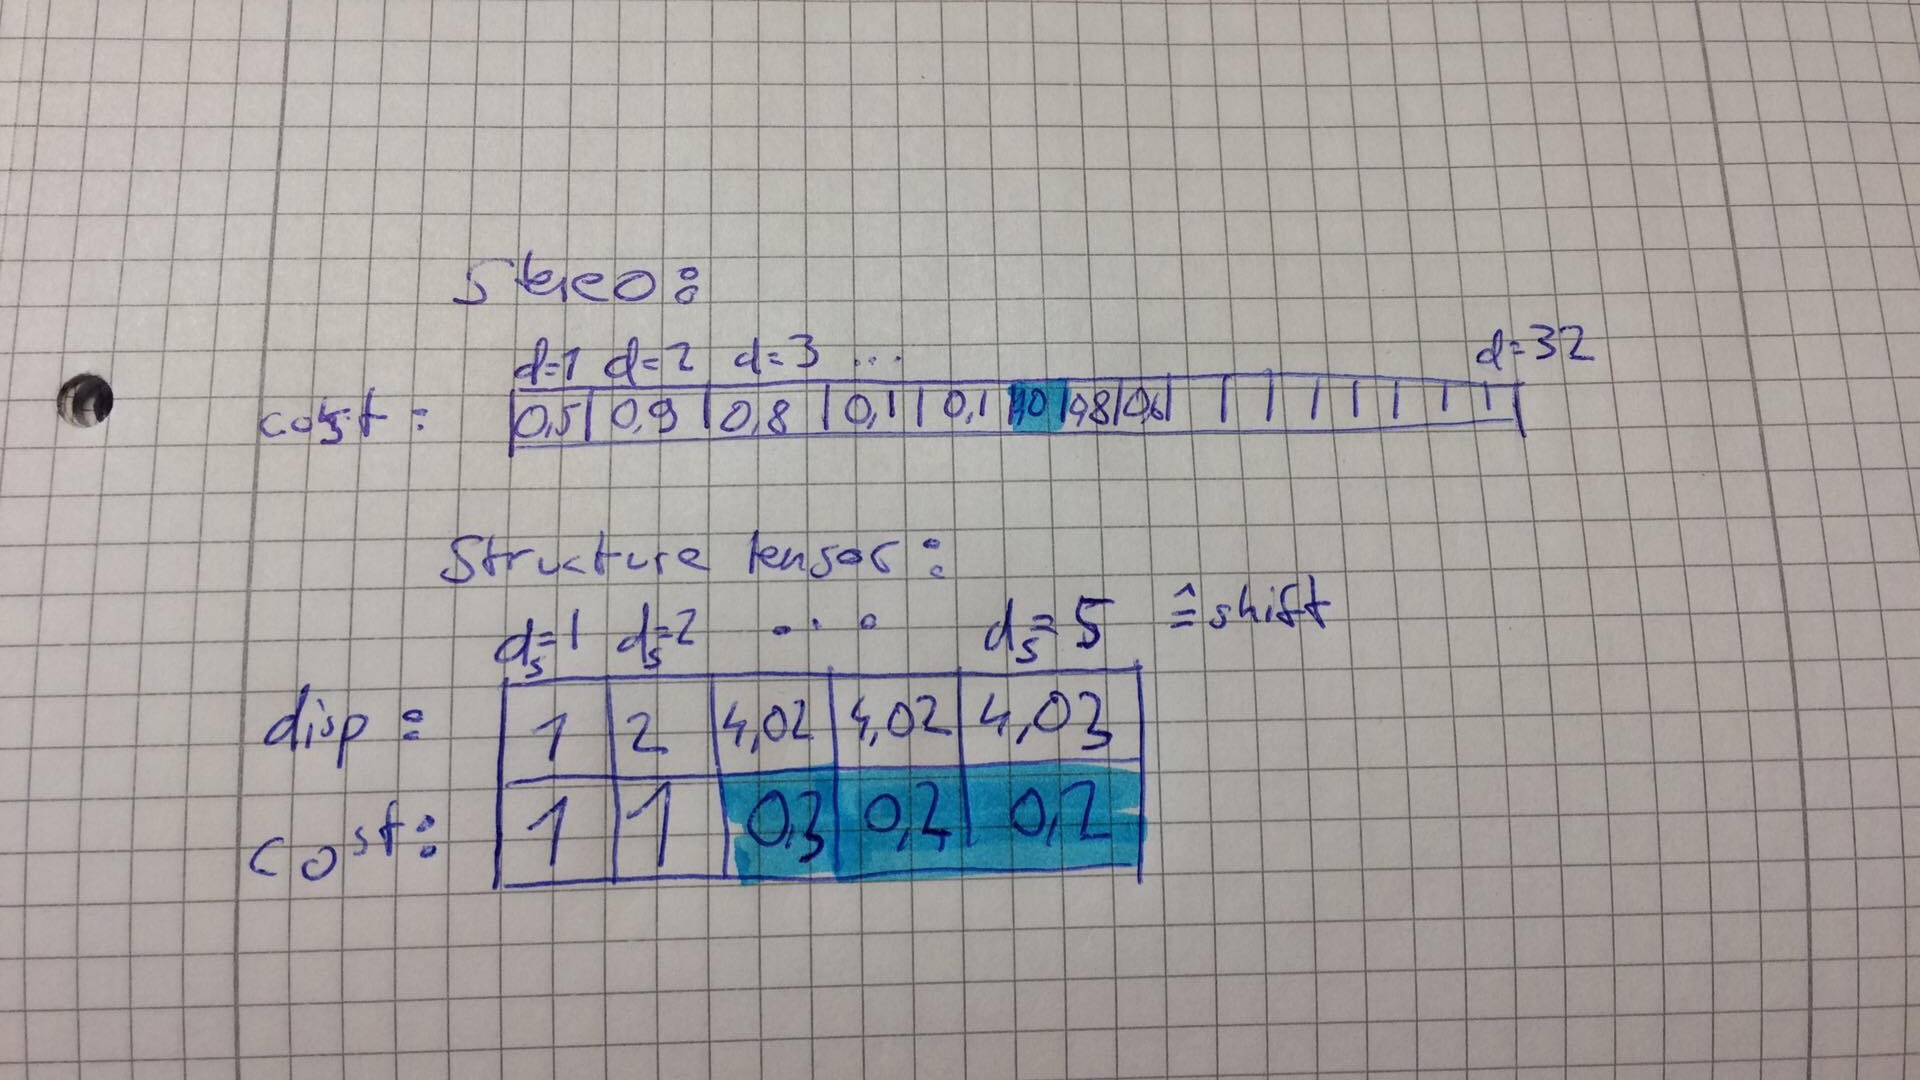
\includegraphics[width=0.7\linewidth]{images/table-skizze}
	\caption[Example values: One point $\vec p$ contains different values]{One point $\vec p$ contains different values (values here: example values): For Stereo matching, the resolution is given by the discrete disparity steps. Each disparity value has a cost value assigned to it. Using the ST, we have a different subpixel accuracy for every disparity shift, while the subpixel accuracy can differ from the shift by up to 1.2 }
	\label{fig:table-skizze}
\end{figure}

To handle those problems, we do not throw away the subpixel accuracy: instead we use the float-value disparities to decide whether we penalize a disparity discontinuity or not. As one can see in figure \ref{fig:table-skizze}, we have to process an additional information, since the exact disparity value is not implicitely given by the index of the allocated cost value (in contrast to the original algorithm). Switching to a continuous space as depicted in figure \ref{fig:discretecont} requires a new definition of the error propagation defined in equation \ref{eq:global_sgm}.
\begin{figure}
	\centering
	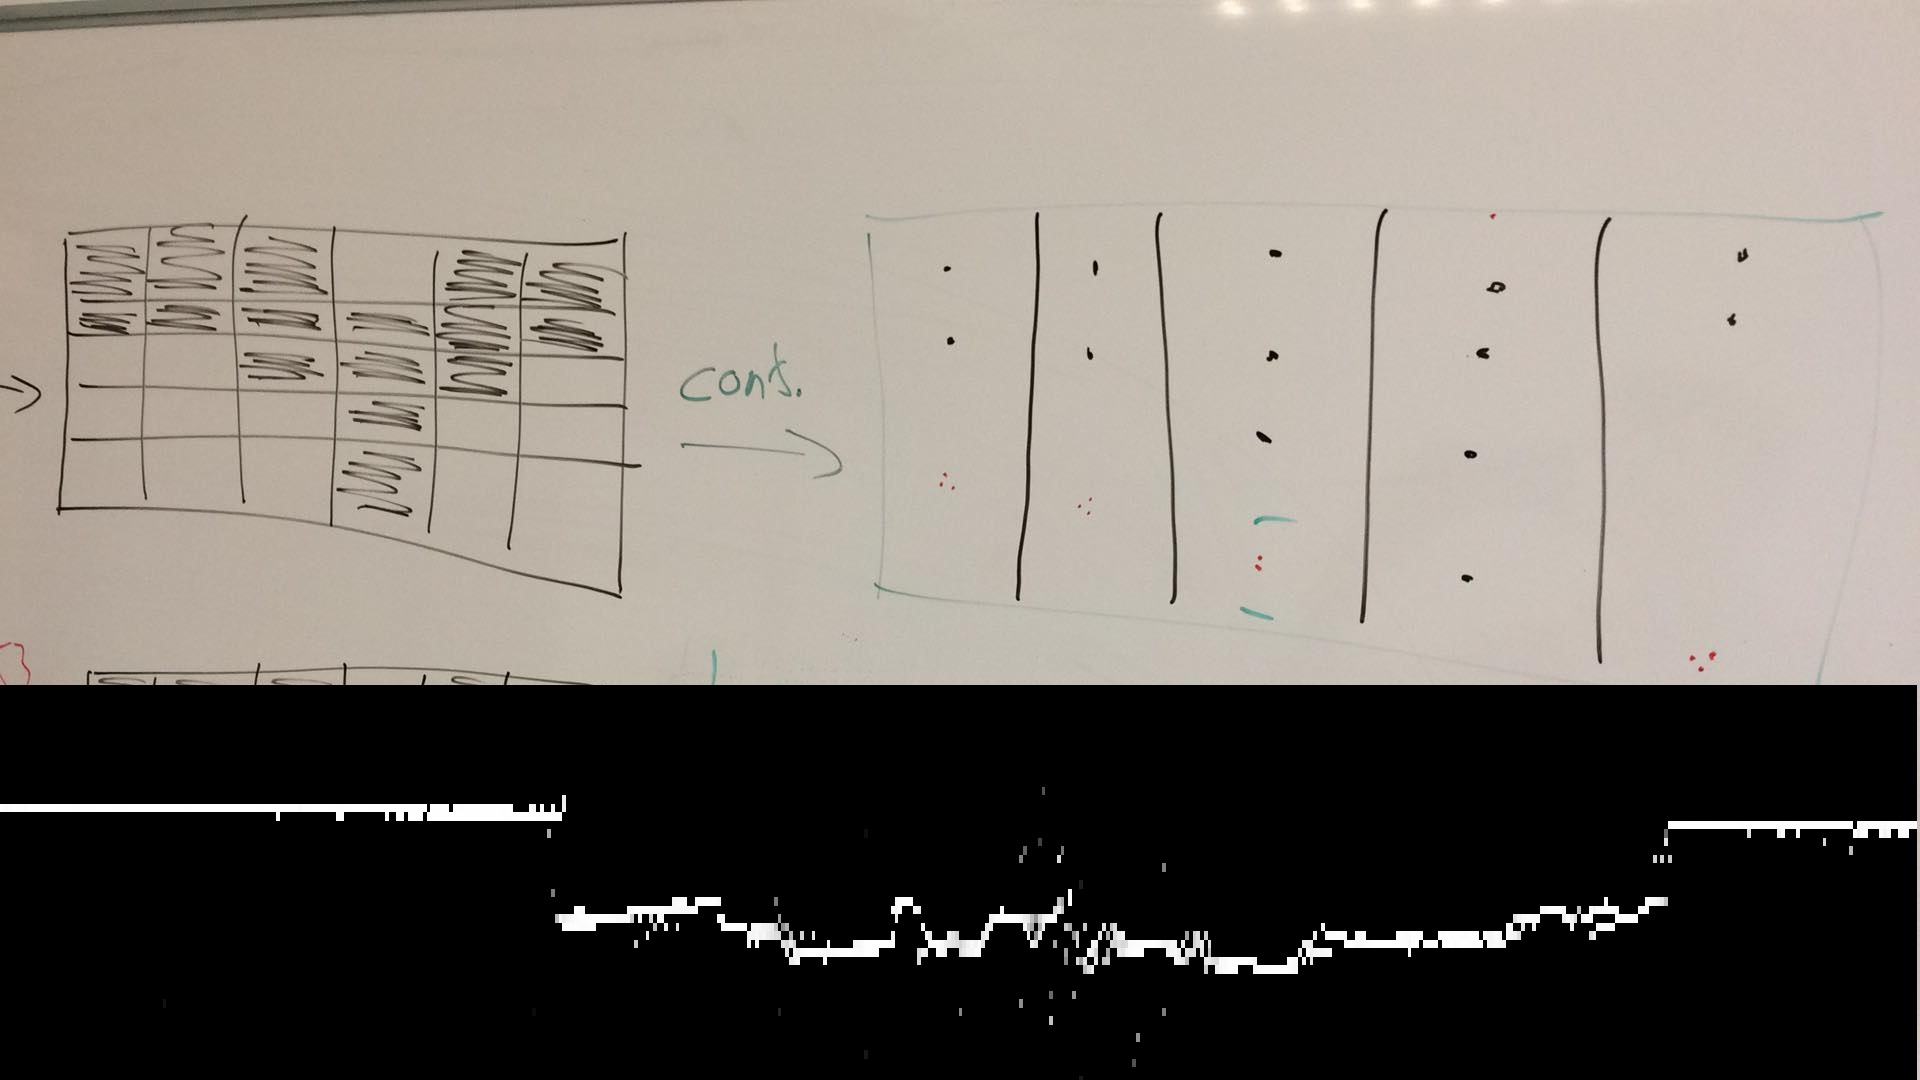
\includegraphics[width=0.7\linewidth]{images/discrete_cont}
	\caption[Discrete scanline to continuous scanline]{In this figure one can see the skizze of one arbitrary scanline of the structure tensor method. Under the Assumption that the ST algorithm recognizes the structure of the EPI perfectly, we either have two or three disparity shifts that have a high coherence (colored white) (a) and result in approximately the same final disparity. This can be seen if we plot the exact disparity values in a continuous space(b). In (c) real data scanline cost is plotted with a resolution of ca. 100 pixels.}
	\label{fig:discretecont}
\end{figure}


 In the following we refer to $s$ as the disparity shift in the ST algorithm. Note that we replaced $D$ by $d$ to clarify that the disparity is no longer discrete:

\begin{equation}\label{eq:global_sgm_cont}
E(d) = \sum_{\vec p} \left(C(\vec{p}, d_{\vec p}) + \sum_{q\in N_p} 
\begin{cases}
P1\cdot |d_{\vec p} - d_{\vec q}|  & \text{ if }|d_{\vec p} - d_{\vec q}| \leq 1\\
P2 & \text{ if }|d_{\vec p} - d_{\vec q}| > 1\\
\end{cases}  
\right).
\end{equation}
The recursive 1-d form to solve the global constraint on a scanline then changes to:

\begin{equation}\label{key}
L'_r(\vec{p}, s) = C(\vec{p}, s) + \text{min}_i
\begin{cases}
L'_r(\vec{p}_\text{before}, s_i)+P1 \cdot |d_{\vec p, s} - d_{\vec{p}_\text{before}, s_i}|  & \text{ if }|d_{\vec p, s} - d_{\vec{p}_\text{before}, s_i}| \leq 1 \\
L'_r(\vec{p}_\text{before}, s_i)+P2 & \text{ if }|d_{\vec p, s} - d_{\vec{p}_\text{before}, s_i}| > 1
\end{cases}
\end{equation} 
The biggest difference lies in the fact that the small factor that is smoothing the image linearely increases with the distance. This change is necessary under the assumption that the disparity space is continuous. In other words we cluster disparity differences between two neighbouring points as either part of one surface ($|d_{\vec p, s} - d_{\vec{p}_\text{before}, s_i}| \leq 1$) that gets smoothed by the linearly increasing penalty, or assume a real disparity discontinuity that is penalized regardless of the size of the jump - the second error remains constant as it is in Stereo matching. Note that in our implementation, $P2$ is modified by 
\begin{equation}\label{key}
P2' =  \frac{P2}{\sqrt{(Im_b^2 +Im_r^2 + Im_g^2)}},
\end{equation}
with $Im$ being the center view of the lightfield and $Im_{b,g,r}$ being the 3 color channels. If the color intensity changes, the penalty for a disparity discontinuity is lowered.

\subsection{Occlusion awareness in SGM for light Fields}
Having a look at the results of the the benchmark test of \cite{honauer2016benchmark} one realizes that most Light field depth estimation algorithms suffer from large errors near depth discontinuities. Since the center view pixels close to the edge of a depth discontinuity are at least partly occluded, this behaviour is to be expected. The ST almost always produces a systematic error near discontinuities, leading to a \glqq magnification \grqq of the object closer to the camera in the depth map, see figure \ref{fig:cottondiscontinuities0070}. We refer to this as \glq qedge fattening \grqq. The reason for this error has its origin in the smoothing of the EPI as part of the algorithm. In figure (INPUT EPI) one can identify that after smoothing , the structure tensor near a occlusion edge calculates the structure of the object in the foreground, since the edge itself is 
If we take a close look at figure \ref{fig:discretecont}, one can see that at least at some discontinuities the ST pipeline manages to calculate the depth of the background structure near boundaries with good coherence, but the foreground structure is overlapping and quantitatively measured with higher coherence. Once we know that at least at some edges an improvement can be made by adapting the evaluation function in a sense that the highest coherence does not necessarily measure the right depth, we realize that SGM is doing the job already. The simple heuristic approach is to change the global minimization function \ref{eq:global_sgm_cont} such that a positive disparity jump is less punished than a negative one. In fact, the function changes to
\begin{equation}\label{eq:global_sgm_cont_occlusion}
E(d) = \sum_{\vec p} \left(C(\vec{p}, d_{\vec p}) + \sum_{q\in N_p} 
\begin{cases}
P1\cdot |d_{\vec p} - d_{\vec q}|  & \text{ if }|d_{\vec p} - d_{\vec q}| \leq 1\\
P2 & \text{ if }d_{\vec p} - d_{\vec q} > 1\\
P3 & \text{ if }d_{\vec p} - d_{\vec q} < -1\\
\end{cases}  
\right).
\end{equation}


\begin{figure}
	\centering
	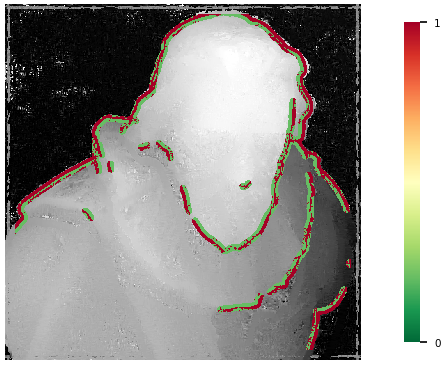
\includegraphics[width=0.7\linewidth]{images/cotton_discontinuities_0070}
	\caption[Discontinuity evaluation]{Evaluation of the deviation from Ground truth at the depth discontinuity for scene "cotton". The red border indicates that the depth map is errorneous at the outside of the edge.}
	\label{fig:cottondiscontinuities0070}
\end{figure}

\chapter{results}
\section{Depth from focus}
\label{sec: depth from focus}
The depth measure using epipolar plane analysis requires iterative calculation of the structure tensor for each EPI at each disparity. A way to overcome this is to generate a preestimate of the depth before actually calculating the correct depth. This could also help to prevent possible errors due to periodic scene characteristics which can lead to mismatch errors when calculating the structure tensor. Therefore the depth pre-estimate should fulfil the following criteria:
\begin{enumerate}
	\item It should be \textit{consistent}, meaning that the number of pixels with low confidence should be the lowest possible.
	\item It should result in a \textit{fast} measure, ideally faster then it would take to do the full iterative structure tensor algorithm.
	\item It does not have to be subpixel accurate, since it only serves as a pre-estimate. 
\end{enumerate}

The methods that are tested are described in section \ref{sec:theo depth}. We test four different ways to obtain a depth map using depth from focus:
\begin{description}
	\item[Photo consistency] This measure takes advantage of the fact that the difference between the refocussed two-dimensional image and the center view is close to zero when refocussed to  the correct depth. Response value:
	\begin{equation}\label{key}
	D'(x,y) = \frac{1}{|W_D|}\sum_{x',y' \in W_D} \left|\bar{L}(x',y')- P(x', y')\right|,
	\end{equation}
	\item[Angular correspondence] In contrast to the \textit{Photo consistency} - measure, it first calculates the absolute difference between each camera array view and the center view followed by the summation of those deviations. The response value is given as in equation \eqref{eq:responsecorr}
	\begin{equation}\label{key}
	D'(x,y) = \frac{1}{N_{u,v}}\sum_{u}\sum_{v}  \left|L'(u, v, x, y) - P(x,y)\right|
	\end{equation}
	
	\item[First derivative] The first derivative is calculated for contrast measure by applying the sobel filter onto the refocussed image $I$:
	\begin{equation}\label{key}
	 G_x=
	 \left[ {\begin{array}{ccc}
	 	-1 & 0 & 1 \\
	 	-2 & 0 & 2 \\
	 	-1 & 0 & 1 \\
	 	\end{array} } \right] \cdot I \quad G_y=
	 \left[ {\begin{array}{ccc}
	 	-1 &-2 &-1 \\
	 	0 & 0 & 0 \\
	 	1 & 0 & 1 \\
	 	\end{array} } \right] \cdot I
	\end{equation} 
	The directional gradients are simply added up to the response value
	\begin{equation}\label{key}
	D'(x,y) = |G_x(x,y)| + |G_y(x,y)|
	\end{equation}
	\item[Laplace] Here we calculate the second derivative laplacian by appling the sobel operator twice:\begin{equation}\label{key}
	D'(x,y) = \text{Laplace}(I)(x,y) = \frac{\partial^2 I}{\partial x^2}(x,y) + \frac{\partial^2 I}{\partial y^2}(x,y)
	\end{equation}
	
	In the following we are going to compare the method qualitatively and quantitatively. In figure \ref{fig:originalmarked} one can see the pixel response value refocussed at different disparities for all the methods at example points in the testscene \glqq complextestscene\grqq. We chose points close to edges as well as points on clear surface with less structure on it. One can see that the pixel response of the Angular correspondence and the Photoconsistency method for those points show a more consistent behaviour, meaning that only one clear maximum can be seen. The derivative method as well as the Laplace method both seem to have trouble especially on pixel coordinates close to edges. This can be seen most clearly at the edge of the melon, where The first derivative shows 2 Maxima, while the Angular correspondence and Photo consistency measure find a clean maximum indicating at which depth the point can be found. However, on surfaces with less structure as for example on the potato, the Photo consistency measure struggles to find a clear maximum -- still it has one at the right position. 
	\begin{figure}
		\centering
		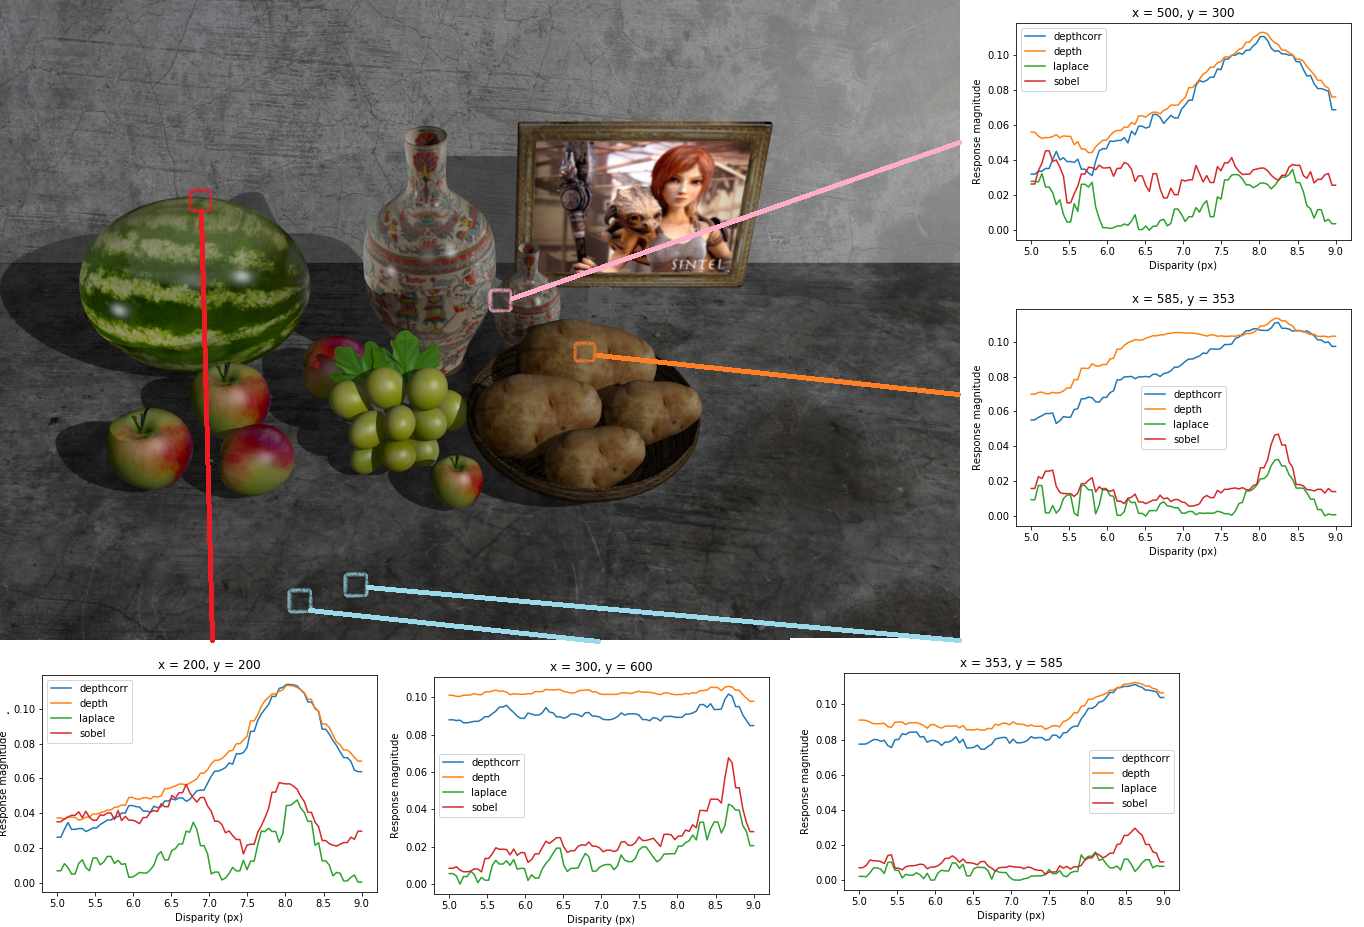
\includegraphics[width=1\linewidth]{images/original_marked}
		\caption[Pixel response for depth from focus techniques]{At different pixel positions we take a look on how the Pixel response value behaves for the four different depth-from-focus techniques: Photo consistency (orange), Angular correspondence ( blue), First derivative (red) and The Laplace method (green) A high value means high confidence (low cost).}
		\label{fig:originalmarked}
	\end{figure}
	Having a look at the actual disparity maps produced by the different techniques we can already
	capture that the angular correspondence and photo consistency method produce the more consistent, smooth disparity maps. A quantitative evaluation confirms this impression: We measure the mean relative error (MRE), which is defined as the mean squared error over all pixels $\vec{p}$ divided by the maximum disparity range (the maximum error possible).
	\begin{equation}\label{key}
	MRE = \sum_{\vec p } (d_{\text{ground truth}} - d_{\vec p} )^2/(\text{max. disp - min. disp})
	\end{equation}
	
	
	
	
	\subsection{Using depth-from-refocus as a preestimate for the ST}
	The long-term aim of this work is to make the structure tensor pipeline more robust. We achieve this by using the depth-from-refocus method as a pre
\end{description}

  \part{Appendix}
  \begin{appendix}
    \chapter{Lists}
    \listoffigures
    \listoftables
    \bibliography{references}{}
    \citestyle{egu}
    \bibliographystyle{plainnat}
    \setlength{\parindent}{0em}

Erkl\"{a}rung:\par
\vspace{3\baselineskip}
Ich versichere, dass ich diese Arbeit selbstst\"{a}ndig verfasst habe und keine
anderen als die angegebenen Quellen und Hilfsmittel benutzt habe.\par
\vspace{5\baselineskip}
Heidelberg, den (Datum)\hspace{3cm}\dotfill

  \end{appendix}
\end{document}
